%%%%%%%%%%%%%%%%%%%%%%%%%%%%%%%%%%%%%%%%%%%%%%%%%%%%%%%%%%%%%%%%%
%																%
% 2. PROJEKT IVS - UŽIVATELSKÁ DOKUMENTACE KALKULACKA			%
% AUTOŘI: Alena Tesarova, Daniel Uhricek, Jan Sorm, Peter Uhrin %
% DATUM: 23.04.2017		
% VERZE: 1.0										%
%																%
%%%%%%%%%%%%%%%%%%%%%%%%%%%%%%%%%%%%%%%%%%%%%%%%%%%%%%%%%%%%%%%%%


\documentclass[11pt,a4paper]{article}
\usepackage[utf8]{inputenc}
\usepackage[left=1.5cm,text={18cm, 25cm},top=2.5cm]{geometry}
\usepackage[czech]{babel}
\usepackage[T1]{fontenc}

\usepackage{times}
\author{Alena Tesařová}
\title{Typografie a publikování - 2. projekt \\
		Sazba dokumentů a matematických vzorců \\}
		
\usepackage{graphicx}
\usepackage{graphics}
\usepackage{picture}
\usepackage{multirow}



\begin{document}

\begin{titlepage}
\begin{center}
\Huge
\textsc{Fakulta informačních technologií\\
Vysoké učení technické v~Brně}\\
\vspace{\stretch{0.382}}

\LARGE \textbf{Uživatelská dokumentace} \\CalculaTron\\

\vspace{\stretch{0.618}}
\end{center}

 \begin{flushright}
 {\Large Daniel Uhříček \\ Alena Tesařová \\Jan Šorm\\ Peter Uhrín \\} 
 \end{flushright}
 {\Large Datum: 23.04.2017 \hfill
 }\\
\end{titlepage}

\newpage
\tableofcontents
\newpage


\section{Důležité informace}
Obsah tohoto manuálu podléhá změnám bez upozornění. Autoři nejsou v žádném případě odpovědní za jakýkoli případ náhodného poškození, které může vzniknout používáním tohoto produktu. Na druhou stranu autoři přijímají jakékoli stížnost a připomínky, které by vedly ke zlepšení jak funkcionality tak grafické stránky produktu. Produkt vznikl jako školní projekt, takže není určen ke komerčnímu využití a software je zakázáno jakkoli šířit bez písemné žádosti autorům produktu.

Ponechte si veškerou uživatelskou dokumentaci při ruce pro budoucí použití.

%doplni Peta
\section{Instalace }

\subsection{Jak nainstalovat}

\subsection{Problémy při instalaci}

\subsection{Odinstalace}

\section{Čtení displeje}
Displej je rozdělen na dvě části - horní a dolní. Hodnota, kterou zrovna zvolíte, se zobrazuje na dolním displeji vpravo. Na horním displeji se nachází celý výpočet i s mezivýpočty. Pokud se výpočet nevleze na šířku displeje, objeví se lišta pro orientaci ve výpočtu. Další informace naleznete v Postupu použití. 

\section{Postup použití - základní výpočty}

%tady bude nase aktualni verze kalkulacky
\begin{figure}[h]
\begin{center}
    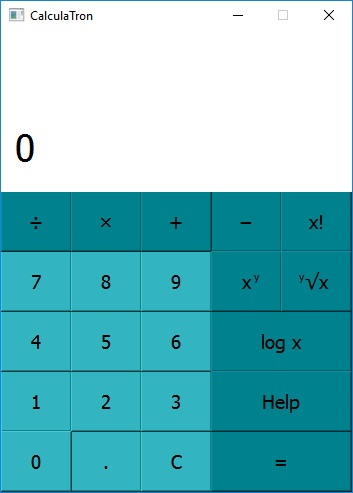
\includegraphics[width=0.3\textwidth,natwidth=610,natheight=642]{calc.png}
    \label{pic:bitmap}
    \caption{CalculaTron}
\end{center}
\end{figure}

Jednotlivé funkce kalkulačky jsou znázorněny na tlačítkách. Pro rychlou orientaci slouží tabulka s vysvětlením jednotlivých funkcí kalkulačky. Nezapomeňte se seznámit s chybovými stavy v kapitole Chyby.

\subsection{Mocnina příklad}
Pro výpočet: $5^3$ 
\begin{enumerate}
\item Zadejte 5
\item Zmáčkněte tlačítko $x^y$
\item Zadejte exponent 3 a pro zobrazení výsledku tlačítko $=$
\item Výsledek se zobrazí na dolním displeji
\end{enumerate}

\subsection{Odmocnina příklad}
Pro výpočet: $\sqrt[3]{9}$ 
\begin{enumerate}
\item Zadejte 9
\item Zmáčkněte tlačítko $\sqrt[y]{x}$
\item Zadejte exponent 3 a pro zobrazení výsledku tlačítko $=$
\item Výsledek se zobrazí na dolním displeji
\end{enumerate}

\subsection{Faktoriál příklad}
Pro výpočet: $3!$ 
\begin{enumerate}
\item Zadejte 3 a tlačítko $x!$
\item Po stisknutí = se výsledek zobrazí na dolním displeji
\end{enumerate}

\subsection{Logaritmus příklad}
Pro výpočet: $log~5$ 
\begin{enumerate}
\item Zadejte 5
\item Zmáčkněte tlačítko $log~x$
\item Po stisknutí = se výsledek zobrazí na dolním displeji
\end{enumerate}


\begin{table}[h]
\begin{center}

\catcode`\-=12 %aby to fungovalo
\begin{tabular}{|c|c|c|} \hline
\label{tab1}
    
     \textbf{Grafické označení}  & \textbf{Vysvětlení} & \textbf{Poznámka}\\ \hline
    $ \div$ & dělení & dělitel nesmí být nula \\
    $\times$ & násobení & \\
    $+$ & sčítání & \\
    $-$ & odčítání & \\
    $x!$ & faktoriál & faktoriál v rozsahu 0--21\\
    $\sqrt[y]{x}$& odmocnina & y $\in N \wedge x \geq 0$\\
    $x^y$& mocnina & y $\in N $\\
    $log~x$& přirozený logaritmus & x > 0\\
    $C$& smazání & vymaže celý výpočet\\
    $.$ & tečka & pro práci s desetinnými čísly\\ \hline
   
\end{tabular}

\caption{ Vysvětlení matematických funkcí CalculaTronu}

\end{center}
\end{table}

%mocnina
%odmocnina
%faktorial
%logaritmus

\section{Chyby}
Kalkulátor zobrazí dialogové okno s chybovým hlášením, kdykoli se během výpočtu objeví chyba. Když je zobrazeno chybové hlášení, stiskněte tlačítko ok pro návrat na obrazovku výpočtu. Uvědomte si také, že tím vymažete výpočet, který obsahoval chybu.

%prosim Honzu o korekci
\subsection{Příčiny chyby}
\begin{itemize}

\item Pokoušíte se dělit nulou
\item Hodnota logaritmu je menší nebo rovna nule
\item Pod sudou odmocninou se nachází záporné číslo
\item Snažíte se zadat zápornou odmocninu
\item Faktoriál není v rozsahu 0 až 21
\item Exponent u mocniny není přirozené číslo
\item Exponent u odmocniny není přirozené číslo
\end{itemize}


\section{Verze}
Jedná se o první verzi kalkulačky 1.0.
\end{document}